\section{100-Semester-Bandverleihung}
\sectionmark{100-Semester-Bandverleihung}

\begin{multicols}{2}
Am 22. März 2024 machten sich Bbr. Philipp Kopystynski und der Verfasser
dieser Zeilen auf nach Vilshofen, um Bbr. Pfarrer Gotthard Weiß sein
längst überfälliges 100-Semesterband zu überreichen. Dies war notwendig,
da der Jubilar gesundheidsbedingt leider nicht mehr nach München reisen
kann. Der Phil-X hat mich dazu dankenswerterweise autorisiert.
Bbr. Weiß wurde am 10. März 1952 geboren und trat nach dem Abitur
unserer lieben Vandalia bei. Die feierliche Reception erfolgte am 17.
November 1971. Geburscht wurde Bbr. Gotthard am 23. Juni 1972. Er
studierte Mathematik für das Lehramt und schloss dieses Studium auch
erfolgreich ab. Doch dann vernahm er den Ruf unseres Herrn und er ging
in seine Heimatdiozöse Passau und nahm das Studium der Theologie auf. In
diesem Zusammenhang war er auch der Gründungssenior der KdStV
Oeno-Danubia zu Passau im CV.
Bbr. Gotthard war vorher auch recht aktiv in der Va: XXXX im WS 72/73, X
im SS 74, FM im WS 74/75. Legendär ist für mich der Mut in das Programm
zu drucken, dass auf dem Haus der Sieg der deutschen
Fussballnationalmannschascht angeschaut und anschließend gefeiert wird.
Ich hätte mich das bei meinen beiden Senioraten nicht getraut. Aber er
hat Recht behalten!
Später gab es tolle Einladungen zu Geburtstagen oder Priesterjubiläen
in  ein jeweils eigens für ihn aufgestelltes Bierzelt. Danke Gotthard,
diese Tage werde ich nie vergessen.
Zwei Jahrzehnte hielt Bbr. Gotthard im Advent Messen in den
Verbindungsräumen der Vandalia. Ich war immer da - in der Regel waren
wir vorher in der Stadt - und werde auch dies nicht vergessen. Aber
daneben ist er auch immer als Seelsorger und Beichtvater für
Bundesbrüder tätig. Es gab jede Menge Aktiven- bzw. Fuxenfahrten zu ihm,
denn er kann auch Bundesbrüder begeistern, die nicht jeden Sonntag in
die Kiche gehen.
Bbr. Gotthard hatte zwei Confüxe, die leider schon verstorben sind:
Norbert Wartha - mein Zipfbruder und Festredner als ich X der Va war -
(2000) und Wilfried Schneider (2023). Lasst uns an sie denken!
Der Tag mit Bbr. Gotthard war sehr schön. Wir sind nach einem
Bergrüßungsbier für mich zu einem schönen Landgasthof in der Nähe
gefahren. Dort fand dann erst die Bandübergabe statt. Der Jubilar
bestand auf einen ordentlichen Streifen aus dem Glas. Dem sind wir
natürlich gerne nachgekommen. Der Wirt wurde vorgewarnt: Wir haben die
Vandalenstrophe geschmettert. Ein anderer Gast hat sogar applaudiert.
Zum Schluss hatt Bbr. Gotthard mir noch seinen Va-Krug mit seinem
Biernamen \glqq Springerl\grqq ~ überreicht, damit ich ihn in der Va an einen
exponierten Platz stelle. Das mache ich natürlich gerne!
Hoffen wir auf viele weitere Bundesbrüder, die unserer Vandalia 50
Jahre, 100 Semester, treu bleiben, damit wir noch viele solche Bänder
verleihen können.
Vivat, crescat, floreat Vandalia ad multos annos!

	\begin{flushright}
		\hfill\emph{Dr. Thomas Strieder AlgA!, Va!, Elb!}
	\end{flushright}
	%	

\end{multicols}

\begin{center}
\begin{figurehere}
		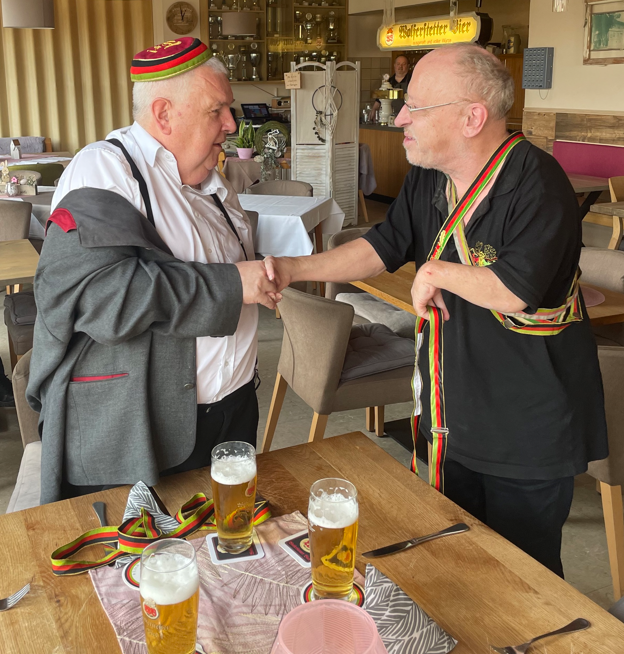
\includegraphics[width=.55\linewidth]{./Bilder/1.4.100Semesterband/2.bild.png} 
\end{figurehere}

\begin{figurehere}
  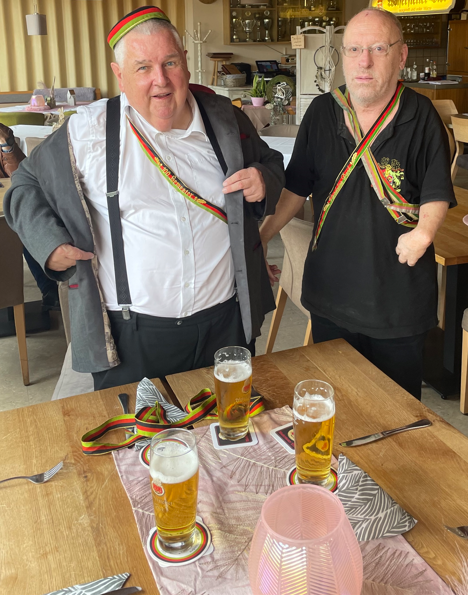
\includegraphics[width=.55\linewidth]{./Bilder/1.4.100Semesterband/1.bild.png} 
  \captionsetup{justification=centering,margin=2cm}
  \caption{Feierliche Bandverleihung an Gotthard Weiß Va! (links) durch\\ ~Dr. Thomas Strieder AlgA! Va! Elb! (rechts)}
\end{figurehere}
\end{center}


%
%\begin{figurehere}
%	\begin{center}
%		\includegraphics[width=.8\linewidth]{Bilder/pios2}
%		\caption{Realer Aufbau} 
%	\end{center}
%\end{figurehere}